\newpage
\section{Network Mapping}

\subsection{Detect the version (30p)}
What type of service is running on kenobi.hackingarena.com in the port range 4500-5000?

\textbf{Solution:}\\
This task was quite straight forward, I used nmap to scan the ports in the range 4500-5000, and got one open port.

\begin{center}
    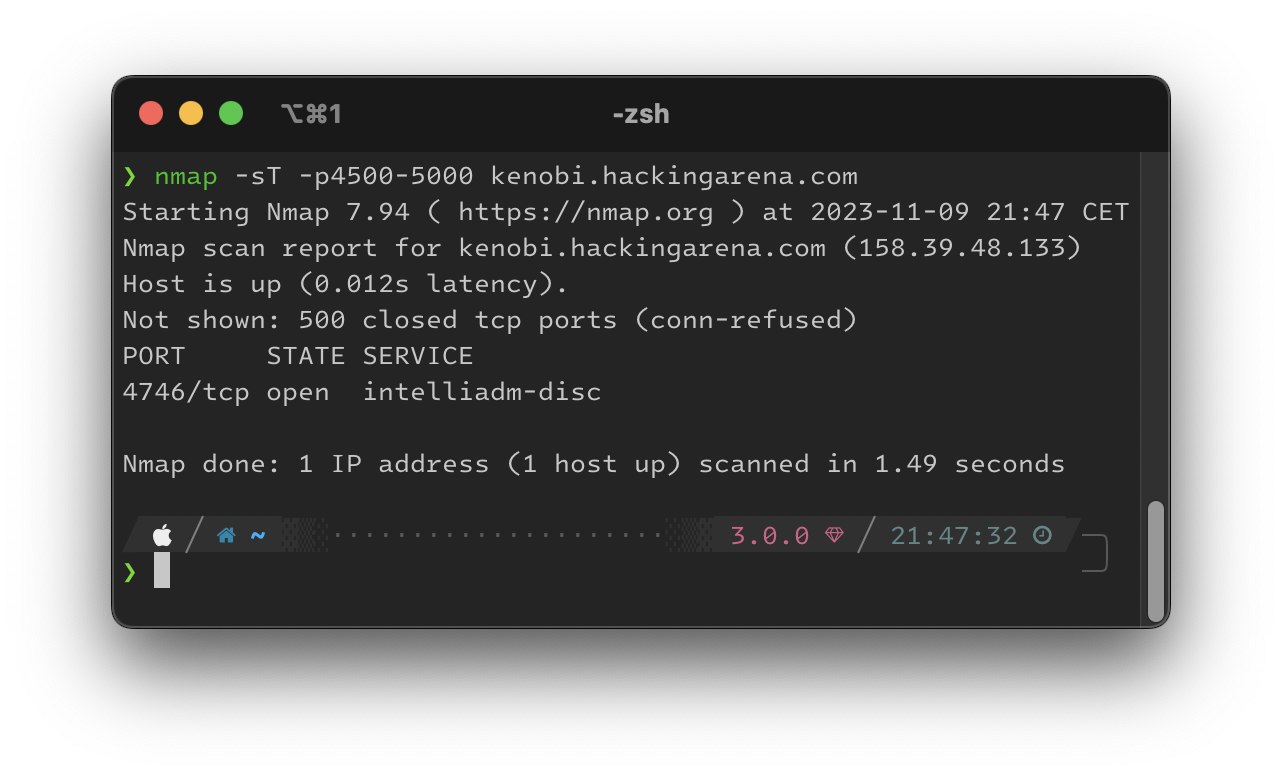
\includegraphics[width=10cm]{img/Network mapping/Detect the version/Screenshot 2023-11-09 at 21.47.37.png}
\end{center}

Then i connected to the address on the specified port with a browser, and got the following page with the answer being ProFTPD:

\begin{center}
    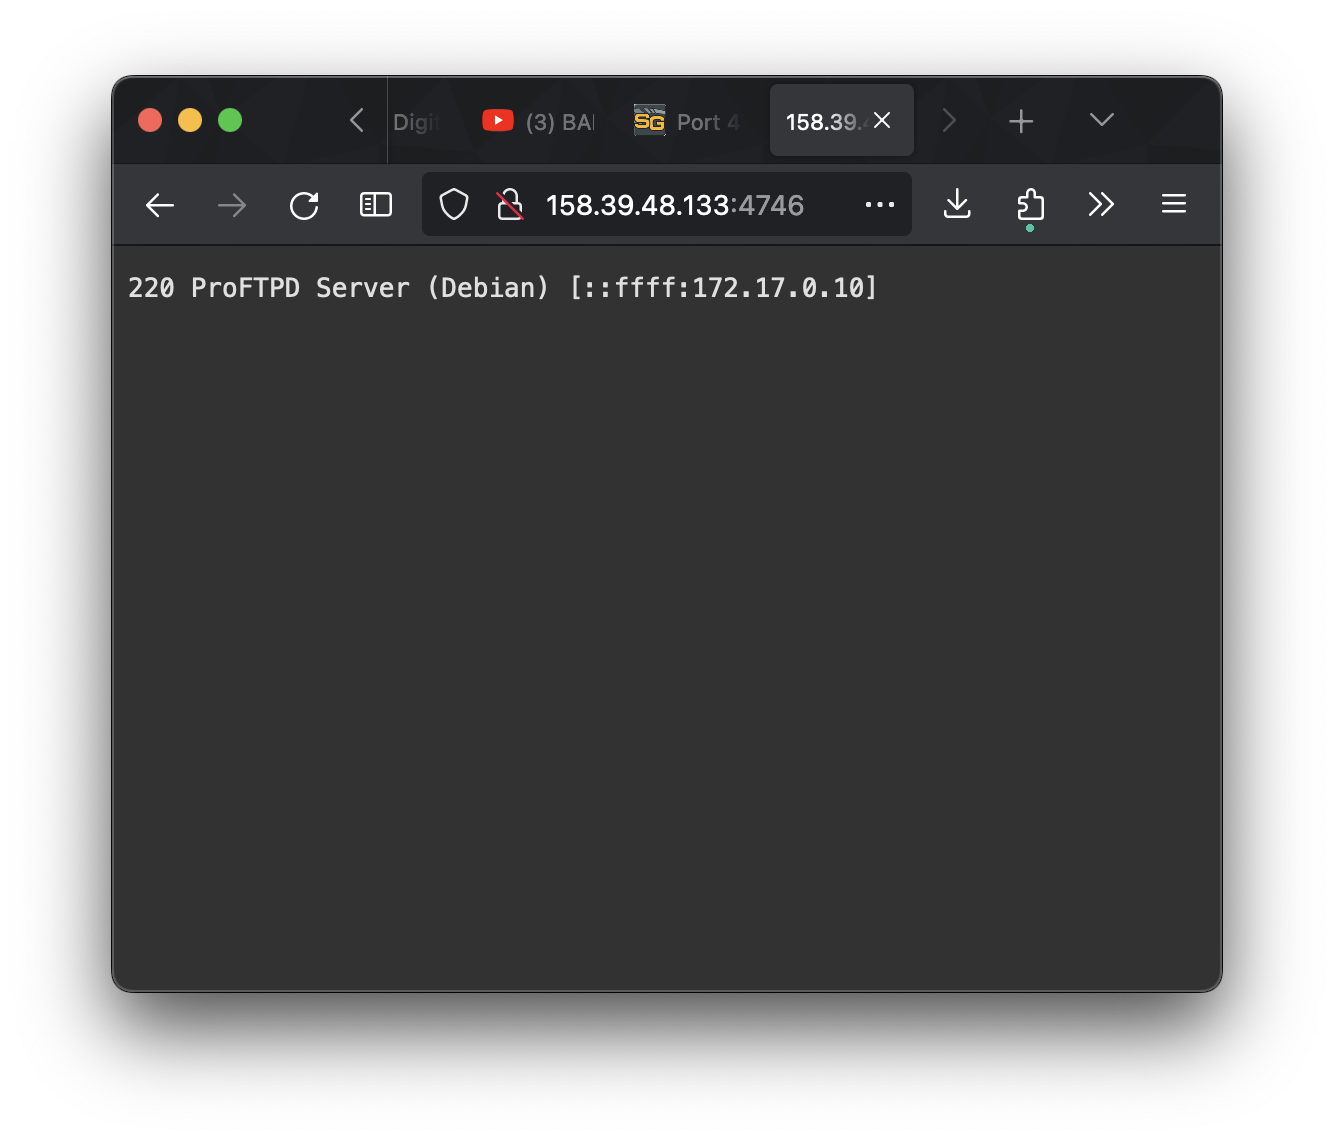
\includegraphics[width=9cm]{img/Network mapping/Detect the version/Skjermbilde 2023-09-10 kl. 19.31.52.png}
\end{center}
    
\newpage
\subsection{Padawan all ports (40p)}
What is the sum of the all open ports at padawan.hackingarena.com? This time not only the regular ports has to be considered. E.g. if only tcp22, tcp80 and tcp443 is open then the answer is 545.

\textbf{Solution:}\\
When I first tried to solve this task i begun a full port scan with nmap using the \texttt{-p-} flag, but after 15 minutes i realised that this would take a long time. So i decided to use the \texttt{-p0-10000} flag to scan the first 10000 ports. This seemed to be enough, as i got the following output:

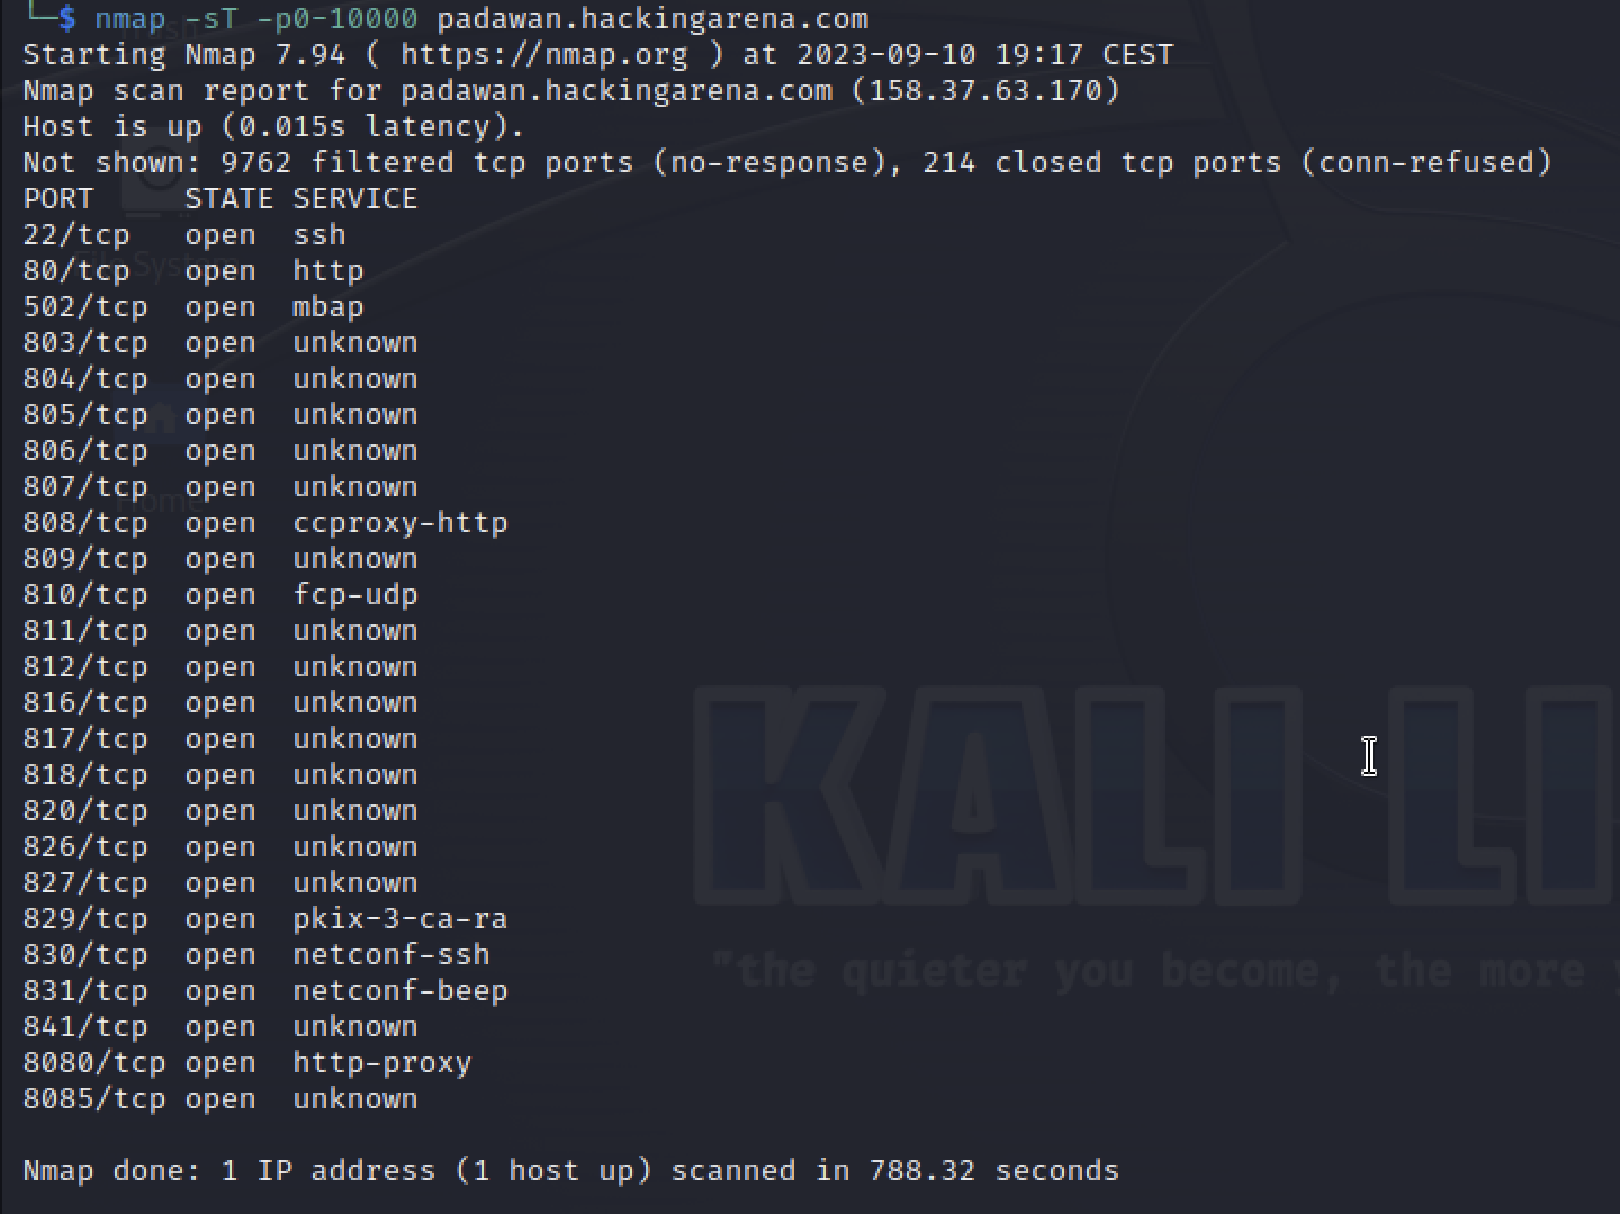
\includegraphics[width=15cm]{img/Network mapping/Padawan all ports/Skjermbilde 2023-09-10 kl. 19.35.19.png}

The sum of all the open ports was 33099.

\newpage
\subsection{Censys (30p)}
Use Censys to find a computer in Oslo that runs Ubuntu 20.04 and tcp port 2233 is open. What is the ip?

\textbf{Solution:}\\
Using Censys I searched for the following query:

\texttt{location.city:oslo and services.port:2233 and services.software.vendor:Ubuntu}

and got the following result:

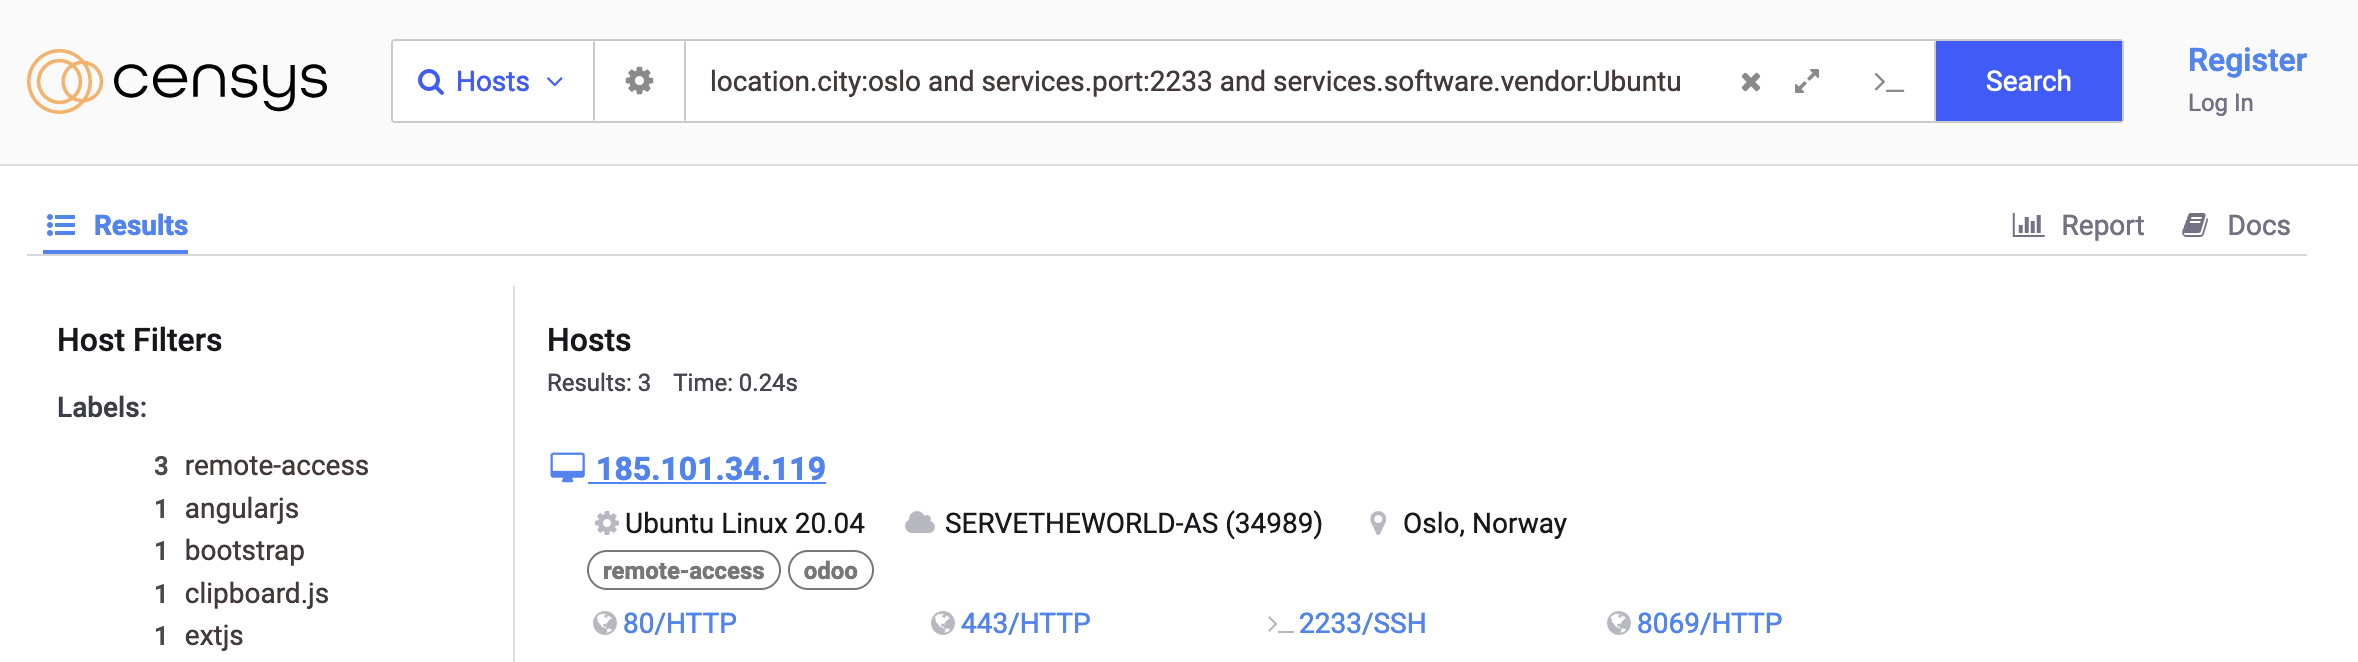
\includegraphics[width=16cm]{img/Network mapping/Censys/Skjermbilde 2023-10-26 kl. 12.40.17.png}

The ip is: \texttt{185.101.34.119}